\chapter{Introducción específica} % Main chapter title

\label{Chapter2}

%----------------------------------------------------------------------------------------
%	SECTION 1
%----------------------------------------------------------------------------------------
Este capítulo introduce las herramientas de terceros y las tecnologías necesarias para el desarrollo del sistema. Se describe la fuente de datos principal, las técnicas para extraer representaciones numéricas del audio, los modelos predictivos y las tecnologías utilizadas para el despliegue.

\section{Fuentes de datos de canciones}
\label{sec:datos}

Para el entrenamiento de los modelos predictivos se utilizó la colección privada de canciones de la empresa. Esta fuente de datos cuenta con más de 60~000 archivos de audio de canciones completas.

Se seleccionó este conjunto de datos por la disponibilidad en el acceso a la información y por su representatividad en ambientes comerciales reales. Por el contrario, otros conjuntos de datos públicos musicales, como GTZAN \citep{GTZAN} y los subconjuntos estándar de FMA \citep{FMA}, ofrecen fragmentos limitados a 10 o 30 segundos de audio. El uso de pistas incompletas restringe la disponibilidad de la información musical. Realizar predicciones sobre el audio total resulta más preciso, ya que evita la pérdida de los eventos musicales que ocurren antes o después de una sola ventana. Además, estas alternativas carecen parcialmente de las variables objetivo requeridas en el alcance del trabajo.

El acceso a los archivos de audio de canciones completas garantiza la preservación de la estructura musical, evita la pérdida de información y flexibiliza la extracción de representaciones matemáticas mediante el uso de bibliotecas y modelos preentrenados.

El análisis comparativo de las fuentes de datos, las representaciones estadísticas de las canciones y los criterios de selección de variables predictivas se detallan en el Capítulo 3.
% TODO: Cambiar "Capítulo 3" por las referencias cruzadas (\ref{}) de las secciones exactas una vez que se termine de escribir el Capítulo 3.

\section{Representaciones numéricas de la música}
\label{sec:dsp}

Una canción se traduce a un formato numérico para su procesamiento computacional. El procesamiento digital de señales (DSP) transforma la onda sonora en arreglos matemáticos de una o dos dimensiones. 
Entre las representaciones bidimensionales más destacadas se encuentran el espectrograma, el cromagrama y el espacio armónico o tonnetz. El espectrograma refleja la variación de las frecuencias a lo largo del tiempo. Por su parte, el cromagrama captura la energía asociada a las doce clases de notas musicales. Finalmente, el tonnetz modela las relaciones tonales y armónicas de la pista. A modo de ejemplo, en la figura \ref{fig:representaciones_2d} se ilustran estas tres transformaciones aplicadas a un fragmento de la canción ``Weird Fishes/Arpeggi'' de la banda Radiohead. En estos gráficos, el eje horizontal representa el tiempo, mientras que la intensidad del color indica la magnitud de la energía para las distintas frecuencias, notas musicales o relaciones tonales correspondientes a cada eje vertical.

\begin{figure}[htpb]
    \centering
    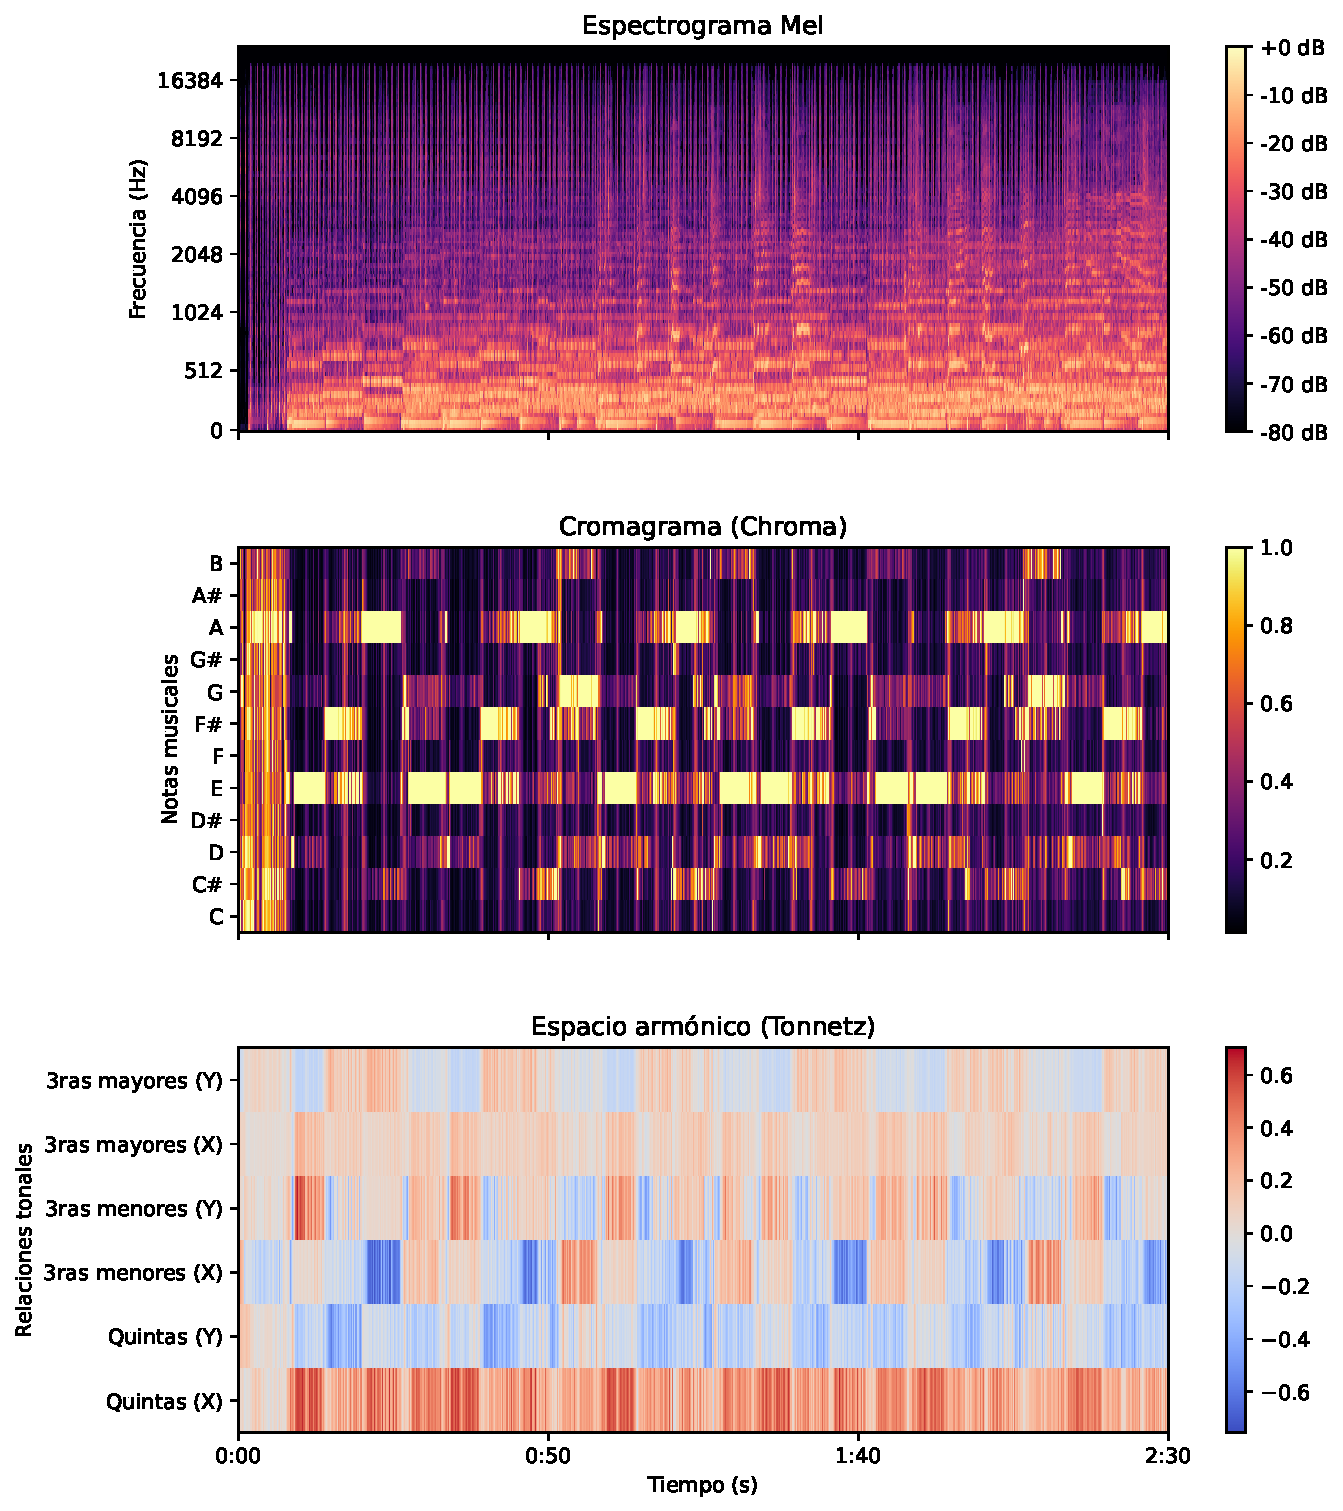
\includegraphics[width=1\textwidth]{./Figures/espectro_croma_tonnetz.pdf}
    \caption[Representaciones visuales del audio]{Representación visual de un espectrograma, un cromagrama y un tonnetz.}
    \label{fig:representaciones_2d}
\end{figure}

Además de las representaciones bidimensionales, las bibliotecas de procesamiento de señales facilitan la extracción de atributos numéricos unidimensionales. En la tabla \ref{tab:atributos_dsp} se presenta un listado que introduce algunas de las características de bajo nivel más representativas en el análisis musical. En la elaboración del trabajo se usaron Librosa y Essentia en este proceso.

Estas transformaciones matemáticas reducen la dimensionalidad del archivo de audio. Sin embargo, carecen de significado semántico. Su función principal, en el contexto de este trabajo, es la de generar las variables predictivas necesarias para entrenar modelos de aprendizaje automático.

El listado completo de las variables de entrada, el análisis de su relevancia y su impacto en el rendimiento de los algoritmos se detalla en el Capítulo 3.

\begin{table}[htpb]
    \centering
    \caption[Atributos representativos]{Listado introductorio de los principales atributos de procesamiento de señales extraídos del audio.}
    \renewcommand{\arraystretch}{1.2}
    \begin{tabular}{p{3.5cm} p{8.5cm}}    
        \toprule
        \textbf{Atributo} & \textbf{Descripción principal} \\
        \midrule
        MFCC & Coeficientes cepstrales que modelan la percepción auditiva humana. \\       
        Centroide espectral & Indica el centro de masa del espectro acústico. Se asocia al brillo del sonido. \\
        Ancho de banda & Mide la dispersión de las frecuencias alrededor del centroide espectral. \\
        Tasa de cruces por cero & Cuantifica la cantidad de cambios de signo en la señal temporal. \\
        Rolloff espectral & Estima la frecuencia por debajo de la que se concentra la mayor parte de la energía. \\
        \bottomrule
    \end{tabular}
    \label{tab:atributos_dsp}
\end{table}

\section{Información semántica del audio}
\label{sec:semantica}

Las representaciones de bajo nivel descritas en la sección 2.2 no siempre son suficientes para capturar conceptos musicales complejos. Es posible mejorar la cobertura de la información musical con el aprendizaje por transferencia. Esta técnica consiste en utilizar modelos previamente entrenados con grandes volúmenes de datos para extraer características semánticas de alto nivel.

Para este fin existen bibliotecas especializadas, como PANNs Inference. Esta herramienta provee acceso a redes neuronales optimizadas para el análisis de eventos sonoros. Dentro de sus opciones, destaca la arquitectura denominada CNN14 \citep{kong2020panns}. Se trata de una red neuronal convolucional, capaz de abstraer patrones del audio y generar embeddings numéricos basados en las clases del conjunto de datos AudioSet. 

Un ejemplo de las probabilidades de detección obtenidas para distintas clases de eventos sonoros a lo largo del tiempo se visualiza en la figura \ref{fig:mapa_semantico}, donde se muestran ventanas consecutivas de 10 segundos de la canción de Radiohead. En este mapa de calor, las áreas más claras indican una mayor probabilidad de activación para cada clase.

El uso de esta arquitectura permite transformar la onda sonora para extraer embeddings y obtener probabilidades asociadas a etiquetas predefinidas, como la presencia de aplausos, instrumentos musicales específicos o habla. Estos datos semánticos enriquecen el conjunto de variables de entrada para la inferencia de algunas de las características musicales que se definieron en el alcance del trabajo.

\newpage
\begin{figure}[!htpb]
    \centering
    
\includegraphics[width=1\textwidth]{mapa_top_clases.pdf}
    \caption[Probabilidades de detección semántica]{Mapa de calor de las características semánticas extraídas mediante la red CNN14.}
    \label{fig:mapa_semantico}
\end{figure}

\section{Modelos de inteligencia artificial utilizados}
\label{sec:modelos}

Una vez obtenidos los descriptores numéricos y semánticos, es necesario aplicar algoritmos de predicción. Para este fin, se utilizaron dos enfoques principales:

\begin{itemize}
    \item Algoritmos LightGBM: se integró la arquitectura LightGBM, basada en el ensamble de árboles de decisión. Esta herramienta destaca por su alta velocidad computacional y eficiencia en tareas generales de predicción.
    \item Redes MLP: los perceptrones multicapa son redes neuronales artificiales con capacidad para modelar relaciones complejas. Permiten, entre otras aplicaciones, predecir múltiples variables continuas de forma simultánea.
\end{itemize}

\section{Despliegue e integración}
\label{sec:despliegue}

La integración del sistema predictivo requirió del despliegue de una interfaz de programación de aplicaciones. Para su construcción se utilizó FastAPI \citep{ramirez2018fastapi} como marco de trabajo. Esta herramienta facilita el desarrollo de servicios web de alto rendimiento basados en Python \citep{python3}.

El alojamiento remoto del producto se apoyó en los servicios de infraestructura de OCI (por su sigla en inglés, Oracle Cloud Infrastructure) \citep{oracle_oci}. Se provisionó una instancia de cómputo virtual en la nube para desplegar la aplicación y ejecutar los modelos predictivos. El uso de esta tecnología garantiza la disponibilidad continua del sistema.

%     \centering
%     \includegraphics[width=0.9\textwidth]{./Figures/diagrama_bloques.pdf}
%     \caption{Diagrama de bloques del sistema en su entorno de despliegue en la nube.}
%     \label{fig:diagrama_despliegue}
% \end{figure}


% \subsection{Uso de mayúscula inicial para los título de secciones}

% Si en el texto se hace alusión a diferentes partes del trabajo referirse a ellas como capítulo, sección o subsección según corresponda. Por ejemplo: ``En el capítulo \ref{Chapter1} se explica tal cosa'', o ``En la sección \ref{sec:ejemplo} se presenta lo que sea'', o ``En la subsección \ref{subsec:ejemplo} se discute otra cosa''.

% Cuando se quiere poner una lista tabulada, se hace así:

% \begin{itemize}
% 	\item Este es el primer elemento de la lista.
% 	\item Este es el segundo elemento de la lista.
% \end{itemize}

% Notar el uso de las mayúsculas y el punto al final de cada elemento.

% Si se desea poner una lista numerada el formato es este:

% \begin{enumerate}
% 	\item Este es el primer elemento de la lista.
% 	\item Este es el segundo elemento de la lista.
% \end{enumerate}

% Notar el uso de las mayúsculas y el punto al final de cada elemento.

% \subsection{Este es el título de una subsección}
% \label{subsec:ejemplo}

% Se recomienda no utilizar \textbf{texto en negritas} en ningún párrafo, ni tampoco texto \underline{subrayado}. En cambio sí se debe utilizar \textit{texto en itálicas} para palabras en un idioma extranjero, al menos la primera vez que aparecen en el texto. En el caso de palabras que estamos inventando se deben utilizar ``comillas'', así como también para citas textuales. Por ejemplo, un \textit{digital filter} es una especie de ``selector'' que permite separar ciertos componentes armónicos en particular.

% La escritura debe ser impersonal. Por ejemplo, no utilizar ``el diseño del firmware lo hice de acuerdo con tal principio'', sino ``el firmware fue diseñado utilizando tal principio''. 

% El trabajo es algo que al momento de escribir la memoria se supone que ya está concluido, entonces todo lo que se refiera a hacer el trabajo se narra en tiempo pasado, porque es algo que ya ocurrió. Por ejemplo, "se diseñó el firmware empleando la técnica de test driven development".

% En cambio, la memoria es algo que está vivo cada vez que el lector la lee. Por eso transcurre siempre en tiempo presente, como por ejemplo:

% ``En el presente capítulo se da una visión global sobre las distintas pruebas realizadas y los resultados obtenidos. Se explica el modo en que fueron llevados a cabo los test unitarios y las pruebas del sistema''.

% Se recomienda no utilizar una sección de glosario sino colocar la descripción de las abreviaturas como parte del mismo cuerpo del texto. Por ejemplo, RTOS (\textit{Real Time Operating System}, Sistema Operativo de Tiempo Real) o en caso de considerarlo apropiado mediante notas a pie de página.

% Si se desea indicar alguna página web utilizar el siguiente formato de referencias bibliográficas, dónde las referencias se detallan en la sección de bibliografía de la memoria, utilizado el formato establecido por IEEE en \citep{IEEE:citation}. Por ejemplo, ``el presente trabajo se basa en la plataforma EDU-CIAA-NXP \citep{CIAA}, la cual...''.

% \subsection{Figuras} 

% Al insertar figuras en la memoria se deben considerar determinadas pautas. Para empezar, usar siempre tipografía claramente legible. Luego, tener claro que \textbf{es incorrecto} escribir por ejemplo esto: ``El diseño elegido es un cuadrado, como se ve en la siguiente figura:''

% \begin{figure}[h]
% \centering
% \includegraphics[scale=.45]{./Figures/cuadradoAzul.png}
% \end{figure}

% La forma correcta de utilizar una figura es con referencias cruzadas, por ejemplo: ``Se eligió utilizar un cuadrado azul para el logo, como puede observarse en la figura \ref{fig:cuadradoAzul}''.

% \begin{figure}[ht]
% 	\centering
% 	\includegraphics[scale=.45]{./Figures/cuadradoAzul.png}
% 	\caption{Ilustración del cuadrado azul que se eligió para el diseño del logo.}
% 	\label{fig:cuadradoAzul}
% \end{figure}

% El texto de las figuras debe estar siempre en español, excepto que se decida reproducir una figura original tomada de alguna referencia. En ese caso la referencia de la cual se tomó la figura debe ser indicada en el epígrafe de la figura e incluida como una nota al pie, como se ilustra en la figura \ref{fig:palabraIngles}.

% \begin{figure}[htpb]
% 	\centering
% 	\includegraphics[scale=.3]{./Figures/word.jpeg}
% 	\caption{Imagen tomada de la página oficial del procesador\protect\footnotemark.}
% 	\label{fig:palabraIngles}
% \end{figure}

% \footnotetext{Imagen tomada de \url{https://goo.gl/images/i7C70w}}

% La figura y el epígrafe deben conformar una unidad cuyo significado principal pueda ser comprendido por el lector sin necesidad de leer el cuerpo central de la memoria. Para eso es necesario que el epígrafe sea todo lo detallado que corresponda y si en la figura se utilizan abreviaturas entonces aclarar su significado en el epígrafe o en la misma figura.



% \begin{figure}[ht]
% 	\centering
% 	\includegraphics[scale=.37]{./Figures/questionMark.png}
% 	\caption{¿Por qué de pronto aparece esta figura?}
% 	\label{fig:questionMark}
% \end{figure}

% Nunca colocar una figura en el documento antes de hacer la primera referencia a ella, como se ilustra con la figura \ref{fig:questionMark}, porque sino el lector no comprenderá por qué de pronto aparece la figura en el documento, lo que distraerá su atención.

% Otra posibilidad es utilizar el entorno \textit{subfigure} para incluir más de una figura, como se puede ver en la figura \ref{fig:three graphs}. Notar que se pueden referenciar también las figuras internas individualmente de esta manera: \ref{fig:1de3}, \ref{fig:2de3} y \ref{fig:3de3}.
 
% \begin{figure}[!htpb]
%      \centering
%      \begin{subfigure}[b]{0.3\textwidth}
%          \centering
%          \includegraphics[width=.65\textwidth]{./Figures/questionMark}
%          \caption{Un caption.}
%          \label{fig:1de3}
%      \end{subfigure}
%      \hfill
%      \begin{subfigure}[b]{0.3\textwidth}
%          \centering
%          \includegraphics[width=.65\textwidth]{./Figures/questionMark}
%          \caption{Otro.}
%          \label{fig:2de3}
%      \end{subfigure}
%      \hfill
%      \begin{subfigure}[b]{0.3\textwidth}
%          \centering
%          \includegraphics[width=.65\textwidth]{./Figures/questionMark}
%          \caption{Y otro más.}
%          \label{fig:3de3}
%      \end{subfigure}
%         \caption{Tres gráficos simples.}
%         \label{fig:three graphs}
% \end{figure}

% El código para generar las imágenes se encuentra disponible para su reutilización en el archivo \file{Chapter2.tex}.

% \subsection{Tablas}

% Para las tablas utilizar el mismo formato que para las figuras, sólo que el epígrafe se debe colocar arriba de la tabla, como se ilustra en la tabla \ref{tab:peces}. Observar que sólo algunas filas van con líneas visibles y notar el uso de las negritas para los encabezados.  La referencia se logra utilizando el comando \verb|\ref{<label>}| donde label debe estar definida dentro del entorno de la tabla.

% \begin{verbatim}
% \begin{table}[h]
% 	\centering
% 	\caption[caption corto]{caption largo más descriptivo}
% 	\begin{tabular}{l c c}    
% 		\toprule
% 		\textbf{Especie}     & \textbf{Tamaño} & \textbf{Valor}\\
% 		\midrule
% 		Amphiprion Ocellaris & 10 cm           & \$ 6.000 \\		
% 		Hepatus Blue Tang    & 15 cm           & \$ 7.000 \\
% 		Zebrasoma Xanthurus  & 12 cm           & \$ 6.800 \\
% 		\bottomrule
% 		\hline
% 	\end{tabular}
% 	\label{tab:peces}
% \end{table}
% \end{verbatim}


% \begin{table}[h]
% 	\centering
% 	\caption[caption corto]{caption largo más descriptivo.}
% 	\begin{tabular}{l c c}    
% 		\toprule
% 		\textbf{Especie} 	 & \textbf{Tamaño} 		& \textbf{Valor}  \\
% 		\midrule
% 		Amphiprion Ocellaris & 10 cm 				& \$ 6.000 \\		
% 		Hepatus Blue Tang	 & 15 cm				& \$ 7.000 \\
% 		Zebrasoma Xanthurus	 & 12 cm				& \$ 6.800 \\
% 		\bottomrule
% 		\hline
% 	\end{tabular}
% 	\label{tab:peces}
% \end{table}

% En cada capítulo se debe reiniciar el número de conteo de las figuras y las tablas, por ejemplo, figura 2.1 o tabla 2.1, pero no se debe reiniciar el conteo en cada sección. Por suerte la plantilla se encarga de esto por nosotros.

% \subsection{Ecuaciones}
% \label{sec:Ecuaciones}

% Al insertar ecuaciones en la memoria dentro de un entorno \textit{equation}, éstas se numeran en forma automática  y se pueden referir al igual que como se hace con las figuras y tablas, por ejemplo ver la ecuación \ref{eq:metric}.

% \begin{equation}
% 	\label{eq:metric}
% 	ds^2 = c^2 dt^2 \left( \frac{d\sigma^2}{1-k\sigma^2} + \sigma^2\left[ d\theta^2 + \sin^2\theta d\phi^2 \right] \right)
% \end{equation}
                                                        
% Para generar la ecuación \ref{eq:metric} se utilizó el siguiente código:

% \begin{verbatim}
% \begin{equation}
% 	\label{eq:metric}
% 	ds^2 = c^2 dt^2 \left( \frac{d\sigma^2}{1-k\sigma^2} + 
% 	\sigma^2\left[ d\theta^2 + 
% 	\sin^2\theta d\phi^2 \right] \right)
% \end{equation}
% \end{verbatim}
